%Text books : \cite{fraleigh}
%Module 1:
%Introduction to extension fields, algebraic extensions, Geometric Constructions Finite fields.
%(Part VI – Section 29, 31 – 31.1 to 31.18, 32, 33 of the text) (20 hours)
%Module 2:
%Unique factorization domains, Euclidean domains. Gaussian integers and multiplicative norms
%(Part IX – Sections 45,46 & 47 of the text) (20 hours)
%Module 3:
%Automorphism of fields, the isomorphism extension theorem , Splitting fields.
%(Part X – Sections 48 & 49, 50 of the text) (25 hours)
%Module 4:
%Separable extensions, Galois Theory, Illustrations of Galois Theory, Cyclotomic Extensions. (mention the insolvability of the quintic)
%( Sections 51, 53, 54, 55 - 55.1 to 55.6 of the text) (25 hours)

% ME010101 Abstract Algebra
%Module 1 - \cite{fraleigh} 11, 14, 16, 17
%Module 2 - \cite{fraleigh} 34, 36, 37
%Module 3 - \cite{fraleigh} 20, 21, 22, 23
%Module 4 - \cite{fraleigh} 24, 26, 27

%Advanced Abstract Algebra
%Module 1 - \cite{fraleigh} 29, 31, 32, 33
%Module 2 - \cite{fraleigh} 45, 46, 47
%Module 3 - \cite{fraleigh} 48, 49, 50
%Module 4 - \cite{fraleigh} 51, 53, 54, 55

%Missing - \cite{fraleigh} 1, 2, 3, 4, 5, 6, 7, 8, 9, 10,
%	12, 13, 15, 18, 19, 25, 28, 30, 35, 38, 39, 40, 41, 42, 43, 44

%Section 29
\section{Extension Fields \S29}
\subsubsection*{Previous Results}
\begin{itemize}
	\item Let $R$ be a commutative ring with unity.
		If $M$ is a maximal ideal in $R$, then $R/M$ is a field.
		\cite[\S27.9]{fraleigh}
	\item Let $F$ be a field.
		Every polynomial in $F[x]$ has a unique factorisation into irreducible polynomials except for order and unit.
		cite[\S27.27]{fraleigh}
	\item If $\alpha$ is a zero of $f(x) \in F[x]$, then $f(\alpha) = 0$.
		cite[\S22.10]{fraleigh}
	\item If $p(x)$ is irreducible over field $F$, then the principal ideal generated by $p(x)$, denoted by $\langle p(x) \rangle$ is a maximal ideal in $F[x]$.
		\cite[\S27.25]{fraleigh}
	\item Let $R$ be a ring with unity.
		And $N$ be an ideal of $R$ containing a unit.
		Then $N = R$.\cite[\S27.5]{fraleigh}
\end{itemize}

\begin{description}
	\item[Basic Goal] Let $F$ be a field and $f(x) \in F[x]$.
	Find a field $E$ such that\\
	$F$ is a subfield of $E$ and there exists a zero of $f(x)$ in $E$ ?
	\item[Extension Field] Let $F$ be a field.
	Field $E$ is an extension field of $F$ if $F$ is a subfield of $E$. \\
	Example : $\mathbb{Q} \le \mathbb{R} \le \mathbb{C}$
	\item[Tower of Fields] A diagrammatic representation emphasising the heirarchy of field extensions in which extension fields appears above their subfields.
\end{description}

\begin{theorem}[Kronecker]
	Let $F$ be field.
	And $f(x)$ be a non-constant polynomial in $F[x]$.
	Then there exists an extension field $E$ of $F$ and an $\alpha \in E$ such that $f(\alpha) = 0$.
\end{theorem}
\begin{proof}
	Let $f(x) \in F[x]$.
	Then $f(x)$ has a unique factorisation into irreducible polynomials in $F[x]$ (except for order and unit).
	Let $p(x)$ be an irreducible factor of $f(x)$.
	If $f(x)$ is irreducible over $F$, then $f(x) = cp(x)$.
	It is enough to construct an extension field $E$ containing both $F$ and $\alpha$ such that ${\color{red}p}(\alpha) = 0$.\\


	If $p(x)$ is irreducible over $F$, then $\langle p(x) \rangle$ is maximal ideal in $F[x]$.
	Therefore, $F[x]/\langle p(x) \rangle$ is a field, say $E$.\\


	Consider the function $\psi : F \to F[x]/\langle p(x) \rangle$ defined by $\psi(a) = a+\langle p(x) \rangle$.
	We claim that $\psi : F \to \psi[F]$ is a field isomorphism.
	$\psi$ is a canonical homomophism with trivial kernel. Thus, $\psi$ is one-to-one.\\


	Let $a,b \in F$.
	And suppose $\psi(a) = \psi(b)$.
	It is enough to prove that $a = b$.
	By the defintion of $\psi$, we have $a+\langle p(x) \rangle = b + \langle p(x) \rangle \implies a-b \in \langle p(x) \rangle$.
	Suppose $a \ne b$.
	Then $a-b \ne 0$ and $degree(a-b) = 0$.
	Then, $\langle p(x) \rangle = F[x]$ which is a contradiction since $\langle p(x) \rangle$ is maximal ideal.
	Therefore, $\psi$ is one-to-one.\\

	
	We have $p(x)$ is a factor of $f(x)$.
	Thus $p(\alpha) = 0 \implies f(\alpha) = 0$.
	Thus, it remains to prove that there exists $\alpha \in F[x]/\langle p(x) \rangle$ such that $p(\alpha) = 0$.\\

	Let $p(x) = a_0 + a_1x + a_2 x^2\cdots + a_n x^n$.
	Consider $\alpha = x + \langle p(x) \rangle$.
	Then $p(\alpha) = \phi_\alpha(p)$.
	Thus, $p(\alpha) = a_0 + a_1(x+\langle p(x) \rangle) + \cdots + a_n(x + \langle p(x) \rangle)^n$.
	Thus, $p(\alpha) = (a_0+a_1x + a_n x^n) + \langle p(x) \rangle = p(x) + \langle p(x) \rangle = \langle p(x) \rangle = 0$.
	Therefore, $p(\alpha) = 0$ and $f(\alpha) = 0$.
\end{proof}

\begin{description}
	\item[algebraic over $F$] Let $F \le E$.
		An element $\alpha \in E$ is algebraic over a field $F$, if there exists $f(x) \in F[x]$ such that $f(\alpha) = 0$.
	\item[transcendental over $F$] Let $F \le E$.
		An element $\alpha \in E$ is transcendental over the field $F$, if it is not algebraic over $F$.
	\item[algebraic number] We have, $\mathbb{Q} \le \mathbb{C}$. A complex number $\alpha \in \mathbb{C}$ is algebraic if  it is algebraic over $\mathbb{Q}$.
		Example : $2,\sqrt{2},i$
	\item[transcendental number] A complex number $\alpha \in \mathbb{C}$ is transcendental if it is not an algebraic number.
		Example : $\pi,e$ (proof excluded)
\end{description}

\textbf{Note 1} : A polynomial $f(x) \in F[x]$ is reducible/irreducible depending upon the choice of the field $F$.
For example : $x^2-2$ is irreducible over $\mathbb{Q}$, but is reducible over $\mathbb{R}$.

\textbf{Note 2} : An element $\alpha \in E$ is algebraic/transcendental depending on the choice of the field $F$.
For example : $\sqrt{2} \in \mathbb{C}$ is algebraic over $\mathbb{Q}$ since $x^2-2 \in \mathbb{Q}[x]$.

\begin{theorem}
	Let $E$ be an extension field of $F$, and $\alpha \in E$.
	Let function $\phi_\alpha : F[x] \to E$ be an evaluation homomoprhism.
	Then $\alpha$ is transcendental  if and only if $\phi_\alpha$ is one-to-one.
\end{theorem}
\begin{proof}
	An element $\alpha \in E$ is transcendental if and only if $f(\alpha) \ne 0$ for any nonzero $f(x) \in F[x]$ where $f(\alpha) = \phi_\alpha(f)$.
	Thus, kernel of $\phi_\alpha$ is trivial.
	That is, $\ker(\phi_\alpha) = \{ 0 \}$.
	Therefore, $\phi_\alpha$ is one-to-one.
\end{proof}

\begin{theorem}
	Let $E$ be an extension field of $F$ and $\alpha \in E$ be algebraic over $F$.
	Then there exists a unique irreducible polynomial $p(x)$ with minimum degree in $F[x]$ and $p(\alpha) = 0$.
	If there exists a nonzero polynomial $f(x) \in F[x]$ with $f(\alpha) = 0$, then $p(x)$ divides $f(x)$.
\end{theorem}
\begin{proof}
	Consider evaluation homomorphism $\phi_\alpha : F[x] \to E$ defined by $\phi_\alpha(f) = f(\alpha)$.
	Then $\ker(\phi)$ is an ideal in $F[x]$.
	Since every ideal in $F[x]$ is principal, there exists $p(x) \in F[x]$ such that $\langle p(x) \rangle = \ker(\phi)$.
	And $f(\alpha) = 0 \implies f \in \ker(\phi) = \langle p(x) \rangle$.
	Thus, $p(x)$ divides $f(x)$.\\

	Suppose $p(x) = r(x)s(x)$.
	Then $p(\alpha) = r(\alpha)s(\alpha) = 0$.
	However, $E$ is a field and has no zero divisors.
	Thus, there exists a polynomial of lesser degree in $\langle p(x) \rangle$ which is a contradiction.
\end{proof}

\begin{description}
	\item[monic polynomial] A polynomial which has $1$ as the coefficient of highest power of $x$.
		For example : $x^3 - 3x \in \mathbb{Q}[x]$
	\item[$irr(\alpha,F)$] The unique monic, irreducible polynomial $p(x) \in F[x]$ such that $p(\alpha) = 0$.
		For example, $irr(\sqrt{3},\mathbb{Q}) = x^2-3$.
		And $\sqrt{3}$ is the \textbf{minimial} polynomial for $\sqrt{3}$ over $\mathbb{Q}$
	\item[$deg(\alpha,F)$] The degree of the unique monic, irreducible polynomial $p(x) \in F[x]$ such that $p(\alpha) = 0$.
		For example, $deg(\sqrt{3},\mathbb{Q}) = 2$.
	\item[simple extension] An extension field $E$ of field $F$ is a simple extension if $E = F(\alpha)$ for some $\alpha \in E$.
\end{description}

\begin{theorem}
	Let $E$ be a simple extension $F(\alpha)$ of field $F$ where $\alpha \in E$ is algebraic over $F$.
	Let $deg(\alpha,F) = n \ge 1$.
	Then any element $\beta \in E$ can be uniquely expressed in the form $\beta = b_0 + b_1\alpha + \cdots + b_{n-1}\alpha^{n-1}$ where $b_k \in F$.
\end{theorem}
\begin{proof}
	Consider the evaluation homomorphism $\phi_\alpha : F[x] \to E$ defined by $\phi_\alpha(f) = f(\alpha)$.
	Then $\phi_\alpha[F[x]] = F(\alpha)$.\\
	
	Let $irr(\alpha,F) = p(x) = x^n + a_{n-1}x^{n-1} + \cdots +a_1x+a_0$.
	Then, $p(\alpha) = 0$.
	Thus, 
\begin{equation}
	\alpha^n = -a_{n-1} \alpha^{n-1}-a_{n-2} \alpha^{n-2} - \cdots - a_1\alpha - a_0
\end{equation}
	Clearly, any higher power of $\alpha$ can be eliminated from $f(\alpha)$ as shown below,
	\begin{align*}
		\alpha^{n+1} = & \alpha \alpha^n = -a_{n-1} \alpha^n -a_{n-2} \alpha^{n-1} - \cdots - a_1\alpha^2 - a_0 \alpha \\ 
		 = & a_{n-1} \left( a_{n-1}\alpha^{n-1}+a_{n-2}\alpha^{n-2}+\cdots+a_1\alpha + a_0 \right)\\
		& - a_{n-2}\alpha^{n-1} - a_{n-3}\alpha^{n-2} - a_1\alpha^2 - a_0 \alpha
	\end{align*}

	Thus, in the representation of the element in $F(\alpha)$, the maximum degree of $\alpha$ is $deg(\alpha,F)-1$.
	Therefore, $\beta \in F(\alpha) \implies \beta = b_0 + b_1\alpha + b_2\alpha^2 + \cdots + b_{n-1}\alpha^{n-1}$.\\

	We can also show that this representation is unique for any $\beta \in F(\alpha)$.
	Suppose $\beta = b_0'+b_1'\alpha+b_2'\alpha^2+\cdots+b_{n-1}'\alpha^{n-1}$.
	Then $0 = (b_0 - b_0') + (b_1 - b_1')\alpha + \cdots + (b_{n-1} - b_{n-1}')\alpha^{n-1} = \phi_\alpha(g)$ where $g(x) = (b_0 - b_0') + (b_1 - b_1')x + \cdots + (b_{n-1} - b_{n-1}')x^{n-1}$.
	Clearly, degree of $g(x)$ is $deg(\alpha,F)-1$ which is less than the minimum degree for a non-zero irreducible polynomial for $\alpha$ over $F$.
	Thus $g(x) = 0$.
	In other words, $b_j = b_j',\ \forall j$ and representation for $\beta \in F(\alpha)$ is unique.
\end{proof}
\subsection{Exercises \S29}
\subsubsection{Irreducibility Conditions for Polynomials}
\begin{enumerate}
	\item Irreducibility over a finite field\\
		$x^2+1$ is irreducible in $\mathbb{Z}_3$ since for every $x \in \{ 0,1,2 \},\ x^2+1 \ne 0$.
\item Irreducibility in rational field : Eisentein's Criteria (\S23.15) \\
	Consider $f(x) = x^3+60x^2+30x+12$ since for $p=3$, $f(x)$ satisfies Eisentein's Criteria.
		And thus is $f(x)$ irreducible over $\mathbb{Q}$.\\
	Note that for $p = 2,5,7,\dots$ the Eisentein's Criteria is not satisified.
\end{enumerate}
\subsubsection{Algebraic over a Field}
\begin{enumerate}
	\item $\sqrt{2}+\sqrt{3}$ is algebraic over $\mathbb{Q}$ \cite[Exercise 29.2]{fraleigh}
	\begin{align*}
		\alpha = & \sqrt{2} + \sqrt{3} \\
		\implies \alpha^2 = & 2 + 2\sqrt{6} + 3 =  5 + 2\sqrt{6}  \\
		\implies \alpha^2 - 5 =  & 2\sqrt{6} \\
		\implies  (\alpha^2-5)^2 = & 24 \\
		\implies \alpha^4 - 10\alpha^2 + 1 = & 0 \\
		\implies \phi_{\alpha}(x^4 - 10x^2 + 1) = & 0 
	\end{align*}
		We have, $irr(\sqrt{2}+\sqrt{3},\mathbb{Q}) = x^{\textcolor{blue}{4}}-10x^2+1$ and $deg(\sqrt{2}+\sqrt{3},\mathbb{Q}) = \textcolor{blue}{4}$.
	\item $\pi,e$ are transcendental numbers. (proof excluded)\\
		However, $\pi$ is algebraic over $\mathbb{Q}(\pi)$ since $x-\pi \in \mathbb{Q}(\pi)[x]$.
		
	\item Consider $\alpha = \pi^2$ and $F = \mathbb{Q}(\pi^3)$. \cite[Exercise 29.16]{fraleigh}
	\begin{align*}
		\alpha^3 = & \pi^6 = (\pi^3)^2 \\
		\alpha^3-(\pi^3)^2 = & 0 \\
		\implies \phi_\alpha(x^3-(\pi^3)^2) = & 0 
	\end{align*}
	Thus, $irr(\pi^2,\mathbb{Q}(\pi^3)) = x^{\textcolor{blue}{3}}-(\pi^3)^2$ and $deg(\pi^2,\mathbb{Q}(\pi^3)) = \textcolor{blue}{3}$.\\ 
		Note that $x^3-(\pi^3)^2 \in \textcolor{blue}{\mathbb{Q}(\pi^3)[x]}$ since $\pi^3 \in \mathbb{Q}(\pi^3) \implies -(\pi^3)^2 \in \mathbb{Q}(\pi^3)$.
		However, $x^3-(\pi^3)^2 \notin \textcolor{blue}{\mathbb{Q}[x]}$.
\end{enumerate}
\subsubsection{Factorisation over Extended Field}
\begin{enumerate}
	\item Factorisation over Finite Extension of Finite Field \cite[Exercise 29.25]{fraleigh}\\
		Let $\alpha$ be a zero of $f(x) = x^3+x^2+1 \in \mathbb{Z}_2[x]$.
		Clearly, $f(x)$ is irreducible over $\mathbb{Z}_2$.
		And $x-\alpha$ is a factor of $f(x)$ in $\mathbb{Z}_2(\alpha)$. We have, $f(x) = (x-a)g(x)$

		$$\text{By long division, } g(x) = \frac{x^3+x^2+1}{x-\alpha} = x^2+(1+\alpha)x+(\alpha+\alpha^2)$$
		Therefore, $x^3+x^2+1 = (x-\alpha)[x^2+(1+\alpha)x+\alpha(1+\alpha)]$.\\

		The elements of $\mathbb{Z}_2(\alpha)$ are of the form $a_0+a_1\alpha+a_2\alpha^2$ where $a_0,a_1,a_2 \in \{0,1\}$.
		Also we have, $\alpha$ is a zero of $x^3+x^2+1$.
		Thus, $\alpha^3 = \alpha^2+1$.\\

		In order to find a zero of $g(x)$ it is sufficient to evaluate $g(x)$ for all the eight elements $ 0, 1, \alpha, (1+\alpha), \alpha^2, (1+\alpha^2),(\alpha+\alpha^2), (1+\alpha+\alpha^2) \in \mathbb{Z}_2(\alpha)$.
		
		Clearly, $g(1) = \alpha^2+2\alpha+2 = \alpha^2$.
		And $g(\alpha) = \alpha^2 + 2\alpha(1+\alpha) = \alpha^2$.
		However, $g(\alpha^2) = \alpha^4+\alpha^3+2\alpha^2+\alpha = \alpha(\alpha^2+1)+(\alpha^2+1) + 0\alpha^2 + \alpha = \alpha^3 + \alpha^2 + 2\alpha + 1 = \alpha^3+\alpha^2+1 = 0$.
		Thus, $\alpha^2$ is a zero of $g(x)$ and $g(x) = (x-\alpha^2)h(x)$.
	$$\text{By long division, } h(x) = \frac{x^2+(1+\alpha)x+(\alpha+\alpha^2)}{x-\alpha^2} = x+(1+\alpha+\alpha^2)$$
		Therefore, we have the following linear factoriation for $f(x)$,\\ $f(x) = (x-\alpha)(x-\alpha^2)(x-1-\alpha-\alpha^2) = (x+\alpha)(x+\alpha^2)(x+1+\alpha+\alpha^2)$ since $-\alpha = 0-\alpha = 2\alpha-\alpha = \alpha$ in $\mathbb{Z}_2$.\\

	Note : Students should be able to perform long division of polynomials over extended fields.
\end{enumerate}

%Section 31
\section{Algebraic Extensions \S31}
\begin{description}
	\item[$(G : H)$] is the number of $H$-left cosets in $G$.
	\item[algebraic extension] A extension field $E$ of a field $F$ is algebraic if every element in $E$ is algebraic over $F$.\\
		For example, $\mathbb{C}$ is algebraic over $\mathbb{R}$.
		But, $\mathbb{R}$ is not algebraic over $\mathbb{Q}$.
	\item[finite extension] A extension field $E$ of field $F$ is a finite extension if $E$ is a finite dimensional vector space over $F$.
		And $[E:F]$ is the \textbf{dimension of the vector space} $E$ over $F$.
		Again, $[E:F]$ is the \textbf{degree of the finite extension} $E$ over $F$.\\
		For example, $\mathbb{C}$ is a finite extension of degree $2$ over $\mathbb{R}$, $[\mathbb{C} : \mathbb{R}] = 2$. But, $\mathbb{R}$ is not a finite extension of $\mathbb{Q}$ and $[\mathbb{R} : \mathbb{Q}]$ is infinite.
\end{description}

\begin{theorem}
	Every finite field extensions is an algebraic extension.
\end{theorem}
\begin{proof}
	Let $E$ be a fintie extension of degree $n$ over $F$.
	Then $[E:F] = n$.
	Suppose $\alpha \in E$.
	Clearly, $\{1,\alpha,\alpha^2,\cdots,\alpha^n \}$ is set of $n+1$ vectors from the vector space $E$ over $F$.
	We know that in a vector space of dimension $n$, any set having $n+1$ vector is linearly dependant.
	In other words, there exits scalars $c_0,c_1,\cdots,c_n \in F$ (not all zero) such that $c_0+c_1\alpha+c_2\alpha^2+\cdots+c_n\alpha^n = 0$.\\

	Clearly, $f(x) = c_0 + c_1x + c_2x^2 + \cdots +c_nx^n$ is a polynomial in $F[x]$ such that $\phi_\alpha(f) = f(\alpha) = 0$.
	Since $\alpha \in E$ is arbitrary, every element in $E$ is algebraic over $F$.
\end{proof}

\begin{theorem}
	If $E$ is a finite extension of $F$ and $K$ is a finite extension of $E$.
	Then $K$ is a finite extension of $F$.
	And $[K:F] = [K:E][E:F]$.
\end{theorem}
\begin{proof}
	Let $[E:F] = n$ and $[K:E] = m$.
	Let $\{ \alpha_1,\alpha_2,\cdots,\alpha_n \}$ be basis for vector space $E(F)$ and let $\{ \beta_1,\beta_2,\cdots,\beta_m\}$ be basis for vector space $K(E)$.
	We claim that $\{\alpha_i\beta_j : 1 \le i \le n,\ 1 \le j \le m \}$ is a basis for the vector space $K(F)$.\\

	Let $\gamma \in K$.
	Then we have $b_1,b_2,\cdots,b_m \in E$ such that $\gamma = b_1\beta_1+b_2\beta_2+\cdots+b_m\beta_m$.
	Again, for each $b_j \in E$, we have $a_{ij} \in F$ such that $b_j = a_{1j}\alpha_1+a_{2j}\alpha_2+\cdots+a_{nj}\alpha_n$.
	Therefore, 
	$$\gamma = \sum_{i=1}^n \sum_{j=1}^m a_{ij} \alpha_i \beta_j$$

	That is, $\{ \alpha_i \beta_j : i =1,2,\cdots,n,\ j=1,2,\cdots,m \}$ spans $K$.
	It remains to prove that $\{\alpha_i \beta_j \}$ is linearly independent.
	Suppose it is linearly dependent.
	Then there exists scalars $c_{i,j} \in F$ (not all zero) such that
	$$\sum_{i=1}^n \sum_{j=1}^m c_{i,j} \alpha_i \beta_j  = \sum_{j=1}^m \left( \sum_{i=1}^n c_{i,j} \alpha_i \right) \beta_j  = 0$$
	
	Let $\sum_{i=1}^n c_{i,j}\alpha_i = b_j$.
	We know that, $\{ \beta_j : j = 1,2,\cdots,m \}$ is linearly independent.
	Thus, $\sum_j b_j \beta_j = 0 \implies b_j = 0,\ \forall j$.\\
	

	Again $b_j = 0 \implies \sum_{i = 0}^n c_{i,j}\alpha_i = 0$.
	Once again, $\{ \alpha_i : i = 1,2,\cdots,n \}$ is linear independent.
	Thus, $c_{i,j} = 0,\ \forall i,j$.
	Thus, $\{ \alpha_i \beta_j \}$ is linearly independent.
	Therefore, $\{ \alpha_i \beta_j \}$ is a basis for the vector space $K(F)$.
	And $[K : F] = |\{\alpha_i \beta_j : i =1,2,\cdots,n \text{ and } j=1,2,\cdots,m\}|= mn$.
\end{proof}

\begin{corollary}
	Let $F_i$ be fields and $F_{i+1}$ are finite extensions of $F_i$s for $i = 1,2,\cdots,r$.
	Then $[F_r : F_1] = [F_r : F_{r-1}][F_{r-1}:F_{r-2}]\cdots[F_2:F_1]$.
\end{corollary}
\begin{proof}
	We have, $F_3$ is a finite extension of $F_1$ and 
	\begin{equation}
		[F_3:F_1] = [F_3:F_2][F_2:F_1]
	\end{equation}
	Suppose $F_k$ is a finite extension of $F_1$ and 
	\begin{equation}
		[F_k : F_1] = [F_k:F_{k-1}][F_{k-1}:F_{k-2}] \cdots [F_2:F_1]
	\end{equation}
	\begin{align*}
		[F_{k+1}:F_1] = & [F_{k+1} : F_k][F_k : F_1] \text{ since } F_k \text{ is a finite extension of } F_1\\
		= & [F_{k+1}:F_k][F_k:F_{k-1}][F_{k-1}:F_{k-2}] \cdots [F_2:F_1]
	\end{align*}
\end{proof}

\begin{corollary}
	If $E$ is an extension field of $F$ and $\alpha \in E$ is algebraic over $F$ and $\beta \in F(\alpha)$, then $deg(\beta,F)$ divides $deg(\alpha,F)$.
\end{corollary}
\begin{proof}
	We have, $\deg(\alpha,F) = [F(\alpha) : F]$ and $\deg(\beta,F) = [F(\beta):F]$.
	Also given that $\beta \in F(\alpha) \implies F(\beta) \le F(\alpha)$.
	Clearly, $F \le F(\beta) \le F(\alpha)$.
	Therefore, $[F(\alpha) : F] = [F(\alpha):F(\beta)][F(\beta):F]$.
	And $[F(\alpha):F(\beta)] = [F(\alpha):F]/[F(\beta):F]$.
	Clearly, $[F(\beta):F]$ divides $[F(\alpha):F]$.
\end{proof}

\begin{theorem}[algebraic closure]
	Let $E$ be an extension field of $F$.
	Then $\bar{F}_E = \{ \alpha \in E : \alpha \text{ is algebraic over } E \}$ is a subfield of $E$.
\end{theorem}
\begin{proof}
	Let $\alpha,\beta \in \bar{F}_E$.
	Then $\alpha,\beta \in E$ are algebraic over $F$.
	And $F(\alpha,\beta)$ is a finite extension field of $F$.
	Thus every element in $F(\alpha,\beta)$ are algebraic over $F$.
	Thus, $\alpha+\beta, \alpha\beta,\alpha-\beta,\alpha/\beta \in \bar{F}_E$.
	Therefore, $\bar{F}_E$ is a subfield of $E$.
\end{proof}

\begin{corollary}
	The set of all algebraic numbers forms a field.
\end{corollary}
\begin{proof}
	Let $\alpha$ be an algebraic number.
	Then $\alpha \in \mathbb{C}$ and $\alpha$ is algebraic over $\mathbb{Q}$.
	Clearly, the set of all algebraic numbers, $\bar{\mathbb{Q}}_\mathbb{C}$ is a subfield of $\mathbb{C}$.
\end{proof}

\begin{description}
	\item[algebraic closure] Let $F$ be a field and $E$ be an extension field of $F$.
		Then the (smallest) field containing all elements of $E$ which are algebraic over $F$ is the algebraic closure $\bar{F}_E$ of $F$ in $E$.
	\item[algebraically closed] Let $F$ be a field.
		$F$ is algebraically closed if every non-constant polynomial in $F[x]$ has a zero in $F[x]$.
		
\end{description}

\textbf{Note : } Let $F$ be algebraically closed.
Then every irreducible polynomial in $F[x]$ are linear since every non-constant polynomial has a linear factor.

\begin{theorem}
	A field $F$ is algebraically closed if and only if every non-constant polynomial $f(x)$ can be factorised in $F[x]$ into linear factors.
\end{theorem}
\begin{proof}
	Let $F$ be algebraically closed and $f(x)$ be a non-constant polynomial in $F[x]$.
	Then $f(x)$ has a zero $\alpha \in F$.
	Then $x-\alpha$ is a factor of $f(x)$.
	That is, $f(x) = (x-\alpha)g(x)$.
	If $g(x) \in F[x]$ is non-constant, then it has a zero in $F$.
	Continuing like this, $f(x)$ can be factorised in $F[x]$ into linear factors.\\

	Suppose every non-constant polynomial in $F[x]$ can be factorised into linear factors.
	Let $f(x)$ be a non-constant polynomial in $F[x]$.
	Then $f(x)$ has a linear factor $(ax+b) \in F[x]$.
	Clearly, $-b/a$ is a zero of $f(x)$.
\end{proof}

\begin{theorem}
	Algebrically closed field has no proper algebraic extensions.
\end{theorem}
\begin{proof}
	Let $E$ be an algebraic extension field of $F$.
	Then if $\alpha \in E$, we have $irr(\alpha,F) = (x-\alpha)$ since $F$ is algebraically closed, every irreduciblepolynomial in $F[x]$ are linear.
	Thus $\alpha \in F$.
	Since $\alpha \in E$ is arbitrary, $F = E$.
\end{proof}

\begin{theorem}[Fundamental Theorem of Algebra]
	$\mathbb{C}$ is algebraically closed.
\end{theorem}
\begin{proof}
	Let $f(z) \in \mathbb{C}[z]$.
	Suppose $f(z)$ has no zeroes in $\mathbb{C}$.
	Then $1/f(z)$ is an entire function and as $|z| \to \infty$, $|f(z)| \to \infty$.
	Thus, $\lim_{|z|\to\infty} \frac{1}{|f(z)|} = 0$.
	And $1/f(z)$ is bounded.\\
	
	By Liouville's theorem, every bounded entire function is constant.
	Therefore, $1/f(z)$ is constant and $f(z)$ is also constant.
	Thus, every non-constant polynomial function in $\mathbb{C}[z]$ has a zero in $\mathbb{C}$.
\end{proof}

\begin{description}
	\item[POSET] Partial Ordered Set - A set together with partial order (reflexive, antisymmetric, transitive relation).\\
		

	For example $(\mathbb{R},<)$, the set of all real numbers together with less than relation is a poset.
		However, in a poset it is not necessary that two arbitrary elements are comparable.
		$(\mathbb{C},R)$ defined by $aRb$ if $\Re(a) = \Re(b)$ and $Im(a) < Im(b)$ is a poset in which $2+3i$ and $3+3i$ are not comparable.
	\item[chain] A subset of a poset in which any two elements are comparable.
		That is, $x,y \in T \implies x < y \text{ OR } y < x$.\\

	For example, For above defined poset $(\mathbb{C},R)$, $T = \{ 2+ib \in \mathbb{C} : b \in \mathbb{R} \}$ is a chain in $\mathbb{C}$.
\end{description}
\begin{lemma}[Zorn]
	If every chain in a poset $S$ has an upper bound.
	Then $S$ has at least one maximal element in it.
\end{lemma}
\begin{proof}
	Not required ( I think, there is no proof.
	We just take it as an axiom - always true !.
	If it is not true for a collection then it is not a set !! )
\end{proof}
\begin{theorem}[Existence of Algebraic Closure]
	Every field $F$ has an algebraic closure $\bar{F}$.
\end{theorem}
\begin{proof}
	Not required (as per syllabus)
\end{proof}
\subsection{Exercise \S31}
\begin{enumerate}
	\item
\end{enumerate}

%Section 32
\section{Geometric Constructions \S32}
\subsection{Basic Constructions}
\subsubsection{Finding Midpoint of a line}
	Let $OA$ be a line.
	The line passing through the intersection of circles with center $O$ and $A$ with diameter greater than the length of the line gives a perpendicular line through its mid point (say, perpendicular bisection).

\subsubsection{Drawing Perpendicular line through a point}
	Let $OA$ be a line and $B$ be a point on that line.
	Find points $P,Q$ on $OA$ which are equidistant from $B$.
	Then the perpendicular bisection of $PQ$ is a line perpendicular to $OA$ through $B$.
\subsubsection{Drawing Parallel Line} 
	Let $OA$ be a line.
	Then the perpendicular line segment of any perpendicular line segment is a line segment parallel to $OA$.
\subsection{Constructible Numbers}
\begin{description}
	\item[Constructible Number] A real number $\alpha$ is constructible if you can draw a line of length $|\alpha|$, given a line of unit length, in finite steps using straightedge and compass.
\end{description}
\begin{theorem}
	Let $\alpha,\beta$ be constructible real numbers.
	Then $\alpha + \beta$, $\alpha-\beta$, $\alpha\beta$, $\alpha/\beta$ ($\beta \ne 0$) are also constructible.
\end{theorem}
\begin{proof}
\begin{description}
	\item[$\alpha+\beta$] Draw a line $OA$ of length $|\alpha|$ and extend that line using straight edge $OE$.
		And draw the line $AB$ of length $|\beta|$ on that extended line, at an point $A$ of the former line extending it.
		Then $OB$ is a line of length $|\alpha| + |\beta|$.
\begin{center}
\begin{tikzpicture}
	\draw[red] (0,0) -- (5,0);
	\draw (0,0) -- (3,0);
	\draw (0,-0.3) node{$O$};
	\draw (3,-0.3) node{$A$};
	\draw (5,-0.3) node{$B$};
\end{tikzpicture}
\end{center}
	\item[$\alpha-\beta$] Draw a line $OA$ of length $|\alpha|$ and extend that line using straight edge $OE$.
		And draw the line $AB$ of length $|\beta|$ on that extended line, at an end point $A$ of former line, but in the opposite direction of extension( towards $O$).
		Then the line $OB$ is of length $|\alpha|-|\beta|$.
\begin{center}
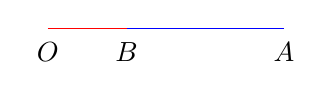
\begin{tikzpicture}
	\draw[blue] (0,0) -- (3,0);
	\draw[red] (0,0) -- (1,0);
	\draw (0,-0.3) node{$O$};
	\draw (3,-0.3) node{$A$};
	\draw (1,-0.3) node{$B$};
\end{tikzpicture}
\end{center}
	\item[$\alpha\beta$] Draw two lines $OA$ and $OB$ of length $|\alpha|$ and $|\beta|$ respectively (with a common end point $O$).
		Now draw the line of unit length $OP$ along the line $OB$.
		Construct triangle $OAP$.
		Draw the line $BQ$ parallel to the line $PA$ through $B$ such that $OQ$ and $OA$ are colinear.
		Now we have two similar triangles $OPA$ and $OBQ$.
		Then, the line $OQ$ of length $\| \alpha \beta \|$.
\begin{center}
\begin{tikzpicture}
	\draw[red] (0,0) -- (6,0);
	\draw (0,0) -- (3,0);
	\draw[blue] (0,0) -- (2.5,2);
	\draw (0,0) -- (1.25,1);
	\draw (2.5,2) -- (6,0);
	\draw (1.25,1) -- (3,0);
	\draw (0,-0.3) node{$O$};
	\draw (3,-0.3) node{$A$};
	\draw (1.25,1.3) node{$P$};
	\draw (2.5,2.3) node{$B$};
	\draw (6,-0.3) node{$Q$};
\end{tikzpicture}
\end{center}
	\item[$\alpha/\beta$] Draw two lines $OA$ and $OB$ of length $\| \alpha \|$ and $\| \beta \|$, with a common end point $O$.
		Draw a line of unit length $OP$ along the line $OB$.
		Now construct triangle $OBA$.
		Draw line $PQ$ parallel to $BA$ so that $OQ$ and $OA$ are colinear.
		Now the triangles $OAB$ and $OQP$ are similar.
		And the line $OQ$ has length $\| \alpha/\beta \|$.
\begin{center}
\begin{tikzpicture}
	\draw[red] (0,0) -- (6,0);
	\draw (0,0) -- (3,0);
	\draw[blue] (0,0) -- (1.5,2);
	\draw (0,0) -- (0.75,1);
	\draw (1.5,2) -- (6,0);
	\draw (0.75,1) -- (3,0);
	\draw (0,-0.3) node{$O$};
	\draw (3,-0.3) node{$Q$};
	\draw (0.60,1.06) node{$P$};
	\draw (1.5,2.3) node{$B$};
	\draw (6,-0.3) node{$A$};
\end{tikzpicture}
\end{center}
\end{description}
\end{proof}

\begin{corollary}
	The set of all constructible real numbers forms a subfield of the field of real numbers.
\end{corollary}
\begin{proof}
	The set of all constructible real numbers say $H$, contains both $0$ and $1$.
	since the line of length zero is trivial and line of unit length is provided.
	And we have, $\forall \alpha,\beta \in H,\ \alpha+\beta,\alpha-\beta,\alpha\beta,\alpha/\beta \in H$.
	Since $\alpha - \beta \in H$, $0-\beta = -\beta$ which is the additive inverse of $\beta$.
	And $1/\beta = \beta^{-1}$ is the multiplicative inverse of $\beta$.
	Thus, the set of all constructible numbers is a subfield of $\mathbb{R}$.
\end{proof}

\begin{theorem}
	The field of $F$ of constructible numbers consists {\color{blue}precisely} of all real numbers that we can obtain from $\mathbb{Q}$ by taking square root of positive numbers a finite number of times and applying a finite number of field operations.
\end{theorem}
\begin{proof}
	The constructible numbers are closed under field operations and forms a subfield $H$ of real numbers.
	We have, $\mathbb{Q}$ is the prime field of $\mathbb{R}$.
	That is, every subfield of $\mathbb{R}$ contains $\mathbb{Q}$.
	Thus, the subfield $H$ of constructible numbers contains $\mathbb{Q}$.
	That is, all the rational numbers are constructible.
	Therefore, it remains to prove that if $\alpha > 0$ is constructible then $\sqrt{\alpha}$ is also constructible.
\begin{center}
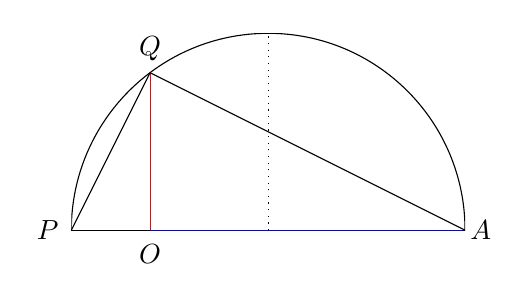
\begin{tikzpicture}
	\draw[blue] (0,0) -- (4,0);
	\draw (0,0) -- (-1,0);
	\draw[red] (0,0) -- (0,2);
	\draw (0,-0.3) node{$O$};
	\draw (4.2,0) node{$A$};
	\draw (-1.3,0) node{$P$};
	\draw (0,2.3) node{$Q$};
	\draw[dotted] (1.5,0) -- (1.5,2.5);
	\begin{scope}
		\clip (-1,0) rectangle (4,2.5);
		\draw (1.5,0) circle (2.5cm);
	\end{scope}
	\draw (4,0) -- (0,2);
	\draw (-1,0) -- (0,2);
\end{tikzpicture}
\end{center}

	Let $OA$ and $OP$ be colinear lines such that $OA$ be a line of length $\| \alpha \|$ and $OP$ be a line of unit length.
	Find the mid point of $PA$ and draw a circle of diameter $PA$.
	Then the length of the perpendicular $OQ$ from $PA$ to the circle is of length $\| \sqrt{\alpha} \|$ since $\Delta OAQ$ and $\Delta OQP$ are similar triangles.\\


	Therefore, real numbers obtained from rational numbers through finite number of additions/subtractions, multplications/divisions, and square root are constructible.
\end{proof}

\textbf{Note : } For example $\sqrt[4]{5\sqrt[8]{3}-2}$ is constructible, but $\sqrt[6]{2}$ and $\pi$ are not constructible.
We skip the proof that a real number which can't be obtained from rationals by a finite number of these operations is not constructible.
And assume that these three operations define the entire field of constructible numbers.

\begin{corollary}
	Let $\gamma$ be constructible number which is not rational.
	Then there exists a sequence of real numbers $\alpha_1,\alpha_2,\dots,\alpha_n = \gamma$ such that for every $i = 2,\dots,n$, the extension field $\mathbb{Q}(\alpha_1,\alpha_2,\dots,\alpha_i)$ is an extension of $\mathbb{Q}(\alpha_1,\alpha_2,\dots,\alpha_{i-1})$ of degree two.\\


	In other words, for any constructible number $\gamma$, $[\mathbb{Q}(\gamma) : \mathbb{Q}] = 2^n$ for some positive integer $n$.
\end{corollary}
\begin{proof}
	Let $\gamma$ be a constructible number which can be obtained from rationals by $n$ square root operations and a finite number of field operations.
	Then, we have a sequence of constructible numbers $\alpha_1, \alpha_2,\dots, \alpha_n$ such that $[\mathbb{Q}(\alpha_1,\alpha_2,\dots,\alpha_i) : \mathbb{Q}(\alpha_1,\alpha_2,\dots,\alpha_{i-1})] = 2$.
	Therefore, $[\mathbb{Q}(\gamma) : \mathbb{Q}] = 2^n$.
\end{proof}

	For example, $\gamma = \sqrt[4]{5\sqrt[8]{3}-2}$.
	Then $\alpha_1 = \sqrt{3}$, $\alpha_2 = \sqrt[4]{3}$, $\alpha_3= \sqrt[8]{3}$, $\alpha_4 = \sqrt{5\sqrt[8]{3}-2}$ and $\alpha_5 = \gamma$.
	Clearly, the geometric construction of $\gamma$ contains five instances of square root operation.

\subsection{Impossible Problems from Ancient Times}
\subsubsection{Doubling the cube}
\begin{theorem}
	There exists a cube such that it is impossible to construct the side of the cube with double the volume.
\end{theorem}
\begin{proof}
	Suppose the cube is of unit side.
	Then the side of the cube with double the volume is $\gamma = \sqrt[3]{2}$.
	And $irr(\gamma,\mathbb{Q}) = x^3-2$ and $[\mathbb{Q}(\sqrt[3]{2}:\mathbb{Q}] = 3 \ne 2^n$.
	Therefore, $\gamma$ is not constructible.
\end{proof}
\subsubsection{Squaring the circle}
\begin{theorem}
	There exists a circle such that it is impossible to construct the side of the square with the same area.
\end{theorem}
\begin{proof}
	Suppose the circle of is of unit radius.
	Then area of the circle is $2\pi$.
	And the side of the square with same area is $\sqrt{2\pi}$.
	Since $\pi$ is transcendental, $\pi$,$\sqrt{\pi}$ and $\sqrt{2\pi}$ are not constructible.
\end{proof}
\subsubsection{Trisecting an angle}
\begin{theorem}
	There exists an angle which can be trisected.
\end{theorem}
\begin{proof}
	We have $\cos 3\theta = 4\cos^3 \theta - 3\cos \theta$.
	Consider $\theta = 20^\circ$.
	Then $\gamma = \cos \theta$ is a root of the irreducible polynomial $4x^3-3x-0.5$.
	That is, $\gamma$ is a root of the monic irreducible polynomial $x^3-\frac{3}{4}x-\frac{1}{8}$ of degree $3$.
	Thus, $\gamma$ is not constructible, since $[\mathbb{Q}(\gamma) : \mathbb{Q}] = 3 \ne 2^n$.
\end{proof}
\subsection{Exercise \S32}
\begin{enumerate}
	\item
\end{enumerate}

%Section 33
\section{Finite Fields \S33}
\subsection{Structure of a Finite Field}
\begin{theorem}
	Let $E$ be a finite extension of degree $n$ over a finite field $F$.
	If $F$ has $q$ elements, then $E$ has $q^n$ elements.
\end{theorem}
\begin{proof}
	We have, extension field $E$ is an $n$-dimensional vector space over the field $F$.
	Let $\{ \alpha_1, \alpha_2,\dots, \alpha_n \}$ be a basis of the vector space $E$ over $F$.
	Then every elements of $E$ can be uniquely written as linear combination of basis vectors.
\begin{equation*}
 	\forall \beta \in E,\ \beta = b_1 \alpha_1 + b_2 \alpha_2 + \dots + b_n \alpha_n
\end{equation*}
	Suppose $\beta \in E$ has two distinct linear combinations.
	Then, the vectors $\{ \alpha_1, \alpha_2,\dots,\alpha_n\}$ are not linearly independent, which is a contatraditciton.\\
	
	Since the reprensentation is unique and $F$ has $q$ elements, there are $q^n$ distinct linear combinations possible.
	Therefore, $E$ has $q^n$ elements.
\end{proof}

\begin{corollary}
	If $E$ is a finite field of characteristic $p$.
	Then $F$ contains exactly $p^n$ elements for some integer $n$.
\end{corollary}
\begin{proof}
	We have, $E$ is a finite field of characteristic $p$.
	Thus, $\mathbb{Z}_p$ is the prime subfield of $E$.
	And $E$ is a finite extension of $\mathbb{Z}_p$.
	Thus, $E$ is a finite dimensional vector space over $\mathbb{Z}_p$.
	Let $n$ be the dimension of $E$ over $\mathbb{Z}_p$.
	And $\mathbb{Z}_p$ has $p$ elements.
	Therefore, $E$ has $p^n$ elements.
\end{proof}

\begin{theorem}
	Let $E$ be a field of $p^n$ elements contained in the algebraic closure $\overline{\mathbb{Z}_p}$ of $\mathbb{Z}_p$.
	Then the elements of $E$ are precisely the zeroes of the polynomial $x^{p^n}-x \in \mathbb{Z}_p[x]$.
\end{theorem}
\begin{proof}
	We have $E^\ast$ is a multiplicative group of non-zero elements in $E$.
	And $E^\ast$ has $p^n-1$ elements.
	Thus, order of any element $\alpha \in E^\ast$ should divide $p^n-1$.
	In other words, if $\alpha \in E^\ast$, then $\alpha^{p^n-1} = 1$.
	Clearly, $\alpha^{p^n} - \alpha = 0$, $\forall \alpha \in E$.
	However, $x^{p^n}$ can have atmost $p^n$ zeroes in $\overline{\mathbb{Z}_p}$.
	Thus, $E$ is precisely the set of all zeroes of $x^{p^n}-x \in \overline{\mathbb{Z}_p}$.
\end{proof}

%\begin{enumerate}[label=Note \arabic*]
%	\item The algebraic closure of $\mathbb{Z}_p$ contains zeroes of every polynomial of the form $x^{p^n}-x$ where $p$ is a prime and $n$ is an integer. Thus, algebraic closures are infinite fields. Remember : $\mathfrak{R}1$
%	\item $\overline{\mathbb{Z}_2}$ has two distinct square roots of unity. And the complex field contains only one of them !
%\end{enumerate}

\begin{description}
	\item[$n$th Root of Unity] $\alpha$ is an $n$th root of unity if $\alpha^n = 1$.
		ie, $\alpha = \sqrt[n]{1}$
	\item[Primitive $n$th Root of Unity] $\alpha$ is a primitive $n$th root of unity if $n$ is the smallest positive integer such that $\alpha^n = 1$.\\
		That is, $\alpha^n = 1$ and $\forall m \in \mathbb{N},\ m < n \implies \alpha^m \ne 1$
\end{description}

\begin{theorem}
	The multiplicative group of non-zero elements of a finite field $F$ is cyclic.
\end{theorem}
\begin{proof}
	Refer : \cite[Theorem 23.6]{fraleigh}
\end{proof}
\begin{corollary}
	Finite extension of finite fields are simple extensions.
\end{corollary}
\begin{proof}
	Let $E$ be a finite extension field of the finite field $F$.
	Then the multiplicative group of non-zero elements $E^\ast$ is cyclic.
	Let $\alpha$ be a generator of the cyclic group $E^\ast$.
	Then, $E = F(\alpha)$.
\end{proof}

\subsection{Galois Field $GF(p^n)$}
\begin{lemma}
	If $F$ is a field of prime characteristic $p$ with algebraic closure $\overline{F}$, then $x^{p^n}-x$ has $p^n$ distinct zeroes in $\overline{F}$.
\end{lemma}
\begin{proof}
	We have, $\overline{F}$ is algebraically closed.
	And $x^{p^n}-x \in \overline{F}[x]$.
	Thus, $x^{p^n}-x$ can be factorised into $p^n$ linear components.
	It remains to prove that these factors are distinct.\\

	Clearly, $0$ is a zero of multiplicity $1$, since $x^{p^n}-x = x (x^{p^n-1}-1)$.
	Let $\alpha \ne 0$ be a zero of $x^{p^n}-x$.
	Then $\alpha$ is a zero of $x^{p^n-1}-1$.
	ie, $\alpha^{p^n-1}  = 1$.
	\begin{align*}
		(x-\alpha)g(x) = & x^{p^n-1}-1 \\
		g(x) = & \frac{x^{p^n-1}-1}{x-\alpha}
		\intertext{By long division, we get}
		g(x) = & x^{p^n-2} + \alpha x^{p^n-3} + \alpha^2 x^{p^n-4} + \dots + \alpha^{p^n-3} x + \alpha^{p^n-2} \\
		g(\alpha) = & (p^n-1)\alpha^{p^n-2} \\
		= &(p^n-1)\frac{\alpha^{p^n-1}}{\alpha} \\
		= & p^n \frac{1}{\alpha} - \frac{1}{\alpha}\\
		= & -\frac{1}{\alpha} \ne 0
	\end{align*}
	Thus, every zero of $x^{p^n-1}-x$ is of multiplicity $1$.
\end{proof}

\begin{lemma}
	If $F$ is a field of prime characteristic $p$, then $(\alpha+\beta)^{p^n} = \alpha^{p^n} + \beta^{p^n}$.
\end{lemma}
\begin{proof}
	Since $F$ is a field of characteristic $p$, for every $\alpha \in F$, $p\alpha = 0$.
	\begin{align*}
		\intertext{ For $n=1$, we have }
		(\alpha+\beta)^p = & \alpha^p + p \alpha^{p-1}\beta+ \frac{p(p-1)}{2} \alpha^{p-2} \beta + \dots + p \alpha \beta^{p-1} + \beta^p \\
		= &  \alpha^p + 0 \alpha^{p-1}\beta+ 0 \alpha^{p-2} \beta + \dots + 0 \alpha \beta^{p-1} + \beta^p \\
		= & \alpha^p + \beta^p
	\end{align*}
	\begin{align*}
		\intertext{Suppose $(\alpha+\beta)^{p^{n-1}} = \alpha^{p^{n-1}} + \beta^{p^{n-1}}$, then} 
		(\alpha+\beta)^{p^n} = & \left[ (\alpha+\beta)^{p^{n-1}} \right]^p \\
		= & \left[ \alpha^{p^{n-1}} + \beta^{p^{n-1}} \right]^p \\
		= & \alpha^{p^n} + \beta^{p^n}
	\end{align*}
	Therefore, by mathematical induction the result is true.
\end{proof}

\begin{theorem}[Existence of Galois Field]
	For every prime power $p^n$, a finite field of $p^n$ elements exists.
\end{theorem}
{\color{blue} Hint : $\alpha^{p^n} = \alpha \iff \alpha^{p^n} - \alpha = 0 \iff \alpha$ is a zero of $x^{p^n} - x$}
\begin{proof}
	Consider the algebraic closure $\overline{\mathbb{Z}_p}$ of $\mathbb{Z}_p$.
	Let $K$ be a subset of $\overline{\mathbb{Z}_p}$ containing all zeroes of $x^{p^n}-x \in \overline{\mathbb{Z}_p}$.\\
	
	Let $\alpha, \beta \in K$.
	Then $\alpha^{p^n} = \alpha$ and $\beta^{p^n} = \beta$.
	Since $\overline{\mathbb{Z}_p}$ is a field of characteristic $p$, we have ${\color{blue}(\alpha+\beta)^{p^n} = \alpha^{p^n}+ \beta^{p^n}} = \alpha + \beta$.
	Thus, $(\alpha+\beta)$ is a zero of $x^{p^n}-x$.
	ie, $(\alpha + \beta) \in K$.
	Clearly, $(\alpha\beta)^{p^n} = \alpha^{p^n} \beta^{p^n} = \alpha\beta$.
	Thus, $\alpha\beta \in K$.\\


	Again $(-\alpha)^{p^n} = (-1 \cdot \alpha)^{p^n} = (-1)^{p^n} \cdot \alpha^{p^n} = -1 \cdot \alpha = -\alpha$.
	Thus, $-\alpha \in K$.
	Also $(\alpha^{-1})^{p^n} = \left( \frac{1}{\alpha} \right)^{p^n} = \frac{1}{\alpha^{p^n}} = \frac{1}{\alpha} = \alpha^{-1}$.
	Thus, $\alpha^{-1} \in K$.\\
	

	Trivially, $0,1 \in K$.
	Therefore, $K$ is a subfield of $\overline{\mathbb{Z}_p}$ with $p^n$ elements since {\color{blue}the $p^n$ zeroes of $x^{p^n}-x$ are distinct}.
\end{proof}

\begin{corollary}
	If $F$ is a finite field, then for every positive integer $n$, there exists an irreducible polynomial in $F[x]$ of degree $n$.
\end{corollary}
\begin{proof}
	Let $F$ be a finite field.
	Then $\mathbb{Z}_p$ is prime field of $F$ for some prime $p$.
	And $F$ is of characteristic $p$ and has $p^r$ elements for some positive integer $r$.\\ %The number of elements of $F$ should be multiple of prime $p$ and shouldn't be a multiple of any other prime $q$.


	Let $K$ be the subfield of $\overline{F}$ containing precisely all the zeroes of the polynomial $x^{p^{rn}}-x \in \mathbb{Z}_p[x]$.
	Then, $K$ has a subfield isomorphic to $\mathbb{Z}_p$ since $F$ is of characteristic $p$ and every subfield of $F$ has a subfield isomorphic to $\mathbb{Z}_p$.\\

	By existence theorem of Galois Fields, every element of $F$ is a zero of the polynomial $x^{p^r}-x \in \mathbb{Z}_p[x]$.
	That is, $\alpha \in F \iff \alpha^{p^r} = \alpha$.
	\begin{align*}
		\alpha^{p^{rn}} & = \left[\alpha^{p^r}\right]^{p^{r(n-1)}} & =  \alpha^{p^{r(n-1)}} & \\
		& = \left[\alpha^{p^r}\right]^{p^{r(n-2)}} & =  \alpha^{p^{r(n-2)}} & \\
		& \vdots & \vdots & \\
		& = \left[\alpha^{p^r}\right]^{p^r} & = \alpha^{p^r} & = \quad \alpha
	\end{align*}
	Thus, $\alpha \in F \implies \alpha^{p^{rn}} = \alpha \implies \alpha \in K$.
	Therefore $F$ is a subfield of $K$.
	Clearly, $K$ is a finite extension of the finite field $F$.
	And the vector space $K$ over $F$ is $n$-dimensional, since $K$ has $p^{rn} = [p^r]^n$ elements and $F$ has $p^r$ elements.\\
	
	Since every finite extension of finite fields are simple extensions, we have $K = F(\beta)$ and $irr(\beta,F) = n$.
	That is, there exists an unique monic, irreducible polynomial $p(x) \in F[x]$ of degree $n$ such that $p(\beta) = 0$.
	Therefore, $\forall n \in \mathbb{Z}^+$, there exists an irreducible polynomial in $F[x]$ of degree $n$.
\end{proof}


\begin{theorem}[Uniqueness of Galois Field]
	Let $p$ be a prime and $n$ a positive integer.
	If $E$ and $E'$ are fields of order $p^n$, then $E$ and $E'$ are isomorphic.\\

	There exists a unique finite field of order $p^n$, say \textbf{Galois Field}, $GF(p^n)$.
\end{theorem}
\begin{proof}
	Let $E,E'$ be fields of order $p^n$.
	Then both fields have $\mathbb{Z}_p$ as prime field.
	Thus, $E$ is a simple extension of $\mathbb{Z}_p$ of degree $n$.
	ie, $[E:\mathbb{Z}_p] = n$.
	And there exits an irreducible polynomial $f(x)$ such that $E \simeq \mathbb{Z}_p[x]/\langle f(x) \rangle$. \\


	Elements of $E$ are zeroes of $x^{p^n}-x$, thus $f(x)$ is a factor of $x^{p^n}-x$.
	Clearly, elements of $E'$ are zeroes of $x^{p^n}$ and therefore $E'$ has all zeroes of $f(x)$.
	And $E' \simeq \mathbb{Z}_p/\langle f(x) \rangle \simeq E$.
	Therefore, there exists a unique field of order $p^n$ (upto isomorphism), say $GF(p^n)$.
\end{proof}

\subsection{Exercise \S33}
\begin{enumerate}
	\item
\end{enumerate}

%Section 45
\section{Unique Factorisation Domains}
\begin{definition}[UFD]
	\textbf{Unique factorisation domain}, UFD is an integral domain such that
	\begin{enumerate}
		\item Every element can be factored into a finite number of irreducibles, except 0 and units
		\dag\footnote{
			Unit is a element which has multiplicative inverse.}.
		\item The above factorisation is unique except for order and associates.
	\end{enumerate}
\end{definition}

For example, In $\mathbb{Z}$, $24 = 2 \times 2 \times 2 \times 3 = -2 \times -3 \times 2 \times 2$.
Here $2$ and $-2$ are associates.
And $2$ and $3$ are not units, since $2^{-1}, 3^{-1} \notin \mathbb{Z}$.

\begin{definition}
	An integral domain is $D$ is a \textbf{Principal Ideal Domain}, PID if every ideal in $D$ is a principal ideal.
\end{definition}[PID]

\subsection{Construction of UFD}
There are two important results on UFDs.
\begin{enumerate}
	\item Every PID is a UFD.
	\item If $D$ is a UFD, then $D[x]$ is a UFD.
\end{enumerate}

\begin{lemma}
	Let $R$ be a commutative ring and let $N_1 \subset N_2 \subset \dots $ be an ascending chain of ideals in $R$.
	Then $N = \cup_i N_i$ is an ideal of $R$.
\end{lemma}
\begin{proof}
\end{proof}

\begin{lemma}[\textbf{A}scending \textbf{C}hain \textbf{C}ondition]
	Let $D$ be a PID.
	If $N_1 \subset N_2 \subset \dots$ is an ascending chain of ideal, then there exists a positive integer $r$ such that $N_r = N_s$ for every $s \ge r$.\\

	In other words, every strictly ascending chain of ideals in a PID is of finite length.
\end{lemma}
\begin{proof}
\end{proof}

\begin{theorem}
	Let $D$ be a PID.
	Every element that is neither $0$ nor a unit in $D$ is a product of irreducibles.
\end{theorem}
\begin{proof}
\end{proof}

\begin{lemma}
	An ideal $\langle p \rangle$ in a PID is maximal if and only if $p$ is an irreducible.
\end{lemma}
\begin{proof}
\end{proof}

\begin{lemma}
	In a PID, if an irreducible $p$ divides $ab$, then either $p|a$ or $p|b$.
\end{lemma}
\begin{proof}
\end{proof}

\begin{corollary}
	If $p$ is an irreducible in a PID $D$ and $p$ divides $a_1a_2\dots a_n$ where $a_i \in D$, then $p|a_i$ for at least one $i$.
\end{corollary}
\begin{proof}
\end{proof}

\begin{definition}
	A nonzero, nonunit element $p$ in an integral domain $D$ is a prime if $\forall a,b \in D,\ p|ab \implies p|a \text{ or } p|b$.
\end{definition}

\begin{theorem}
	Every PID is a UFD.
\end{theorem}
\begin{proof}
\end{proof}

\begin{corollary}
	The integral domain $\mathbb{Z}$ is a UFD.
\end{corollary}
\begin{proof}
\end{proof}

\begin{definition}
	Let $D$ be a UFD and $a_1,a_2,\dots,a_n$ be nonzero elements in $D$.
	An element $d \in D$ is a \textbf{g}reatest \textbf{c}ommon \textbf{d}ivisor of $a_i$ if $d$ is a common divisor of all $a_i$s and also divides any common divisor of $a_i$s.
\end{definition}

\begin{definition}
	Let $D$ be a UFD.
	A noncontant polynomial $a_0 + a_1x + \dots + a_nx^n \in D[x]$ is a primitive if $1$ is the gcd of all $a_i$s.
\end{definition}
	For exmaple, $4x^3+3x^2+2 \in \mathbb{Z}[x]$ is a primitive since $\gcd(4,3,2) = 1$.

\begin{lemma}
	If $D$ is a UFD, then for every nonconstant $f(x) \in D[x]$ we have $f(x) = cg(x)$ where $c \in D$ and $g(x) \in D[x]$ and $g(x)$ is primitive.
	The element $c \in D$ is unique upto a unit factor in $D$ and is the \textbf{content} of $f(x)$.
	Also $g(x)$ is unique upto a unit factor in $D$.
\end{lemma}
\begin{proof}
\end{proof}

\begin{lemma}[Gauss]
	If $D$ is a UFD, then product of two primitive polynomials in $D[x]$ is again primitive.
\end{lemma}
\begin{proof}
\end{proof}

\begin{corollary}
	If $D$ is a UFD, then a finite product of primitive polynomials in $D[x]$ is again primitive.
\end{corollary}
\begin{proof}
\end{proof}

\begin{lemma}
	Let $D$ be a UFD and let $F$ be a field of quotients of $D$.
	Let $f(x) \in D[x]$ where $\deg f(x) > 0$.
	If $f(x)$ is an irreducible in $D[x]$, then $f(x)$ is also an irreducible in $F[x]$.
	Also, if $f(x)$ is primitive in $D[x]$ and irreducible in $F[x]$, then $f(x)$ is irreducible in $D[x]$.
\end{lemma}
\begin{proof}
\end{proof}

\begin{corollary}
	If $D$ is a UFD and $F$ is a field of quotients of $D$, then a nonconstant polynomial $f(x) \in D[x]$ factors into a product of two polynomials of lower degrees $r$ and $s$ in $F[x]$ if and only if it has a factorization into polynomials of the same degress $r$ and $s$.
\end{corollary}
\begin{proof}
\end{proof}

\begin{theorem}
	If $D$ is a UFD, then $D[x]$ is a UFD.
\end{theorem}
\begin{proof}
\end{proof}

For example, let $x,y$ be two indeterminates, then an element $f(x) \in F[x,y]$ is of the form $\displaystyle\sum_{i,j = 0}^{n,m} a_{ij}x^i y^j$.

\begin{corollary}
	If $F$ is a field of quotients and $x_1,x_2,\dots,x_n$ are indeterminates, then $F[x_1,x_2,\dots,x_n]$ is a UFD.
\end{corollary}
\begin{proof}
\end{proof}

\subsection{Exercise \S45}
\begin{enumerate}
	\item
\end{enumerate}


